\chapter{Simulation Work} % (fold)
\label{cha:simulations}
In thesis, the 2D FPE theory is extended for 3D bipedal robots by selecting a sagittal plane in 3D space and constraining the swing foot motion within this plane. Once the biped is unstable, we solve FPE equation along the selected plane to determine the swing foot placement to ultimately regain stability. Similar to the approach used in \cite{Wight:2008ii,Wight:2008vt}, we extend this concept to form complete gait cycles with a state machine, high gain PD controllers and no precomputed trajectories.

\section{Foot Placement Estimator in 2D} % (fold)
\label{sec:foot_placement_estimator_in_2d}
In this section, the FPE approach for 2D systems initially developed by Dwight et al. \cite{Wight:2008ii} is briefly reviewed. The derivation of the underlying theory begins with the simple biped model as shown in Figure~\ref{fig:unified}. The physical parameters are the mass $m$, inertia about the center of mass $I_{COM}$, fixed leg lengths $L$ and leg separation angle $\beta$. By imposing the geometric constraints that $\beta$ is fixed and there is no slipping at the contact points, a single state variable $\theta$ is used to completely define the motion of the compass biped:

\begin{figure}[!h]
	\centering
    \includegraphics[scale=0.7]{fig/ch4/compass.pdf}
  	\caption{Unified variable $\theta$ used to simplify the analysis. It is easily observed that $\theta_A = \theta  + \beta /2$ and $\theta_B = \theta  - \beta /2$}.
	\label{fig:unified}
\end{figure}

The impact of the contact points with the ground is modelled using the conservation of angular momentum to determine the regions in the state space where the biped remains stable after ground contact, by analyzing the total system energy post impact. The stability analysis is then used to determine where a biped must step to remain within the stability region. This forms the basis of the FPE, which is a point on the ground where, if the robot were to step onto that point, the kinetic energy of the biped system would equal the peak potential energy. Placing the swing foot beyond the FPE point results in the biped not having enough kinetic energy post impact to overcome the peak potential energy. In this case, the biped remains stable. Conversely, placing the swing foot before the FPE point causes the kinetic energy post impact to exceed the peak potential energy. In this situation the biped begins to fall over.

\begin{subnumcases}{\ddot{\theta}=\label{eom}}
	\frac{{mgL\sin (\theta  + \beta /2)}}{{{I_{COM}} + m{L^2}}} & $\theta < 0$ \\
	\frac{{mgL\sin (\theta  - \beta /2)}}{{{I_{COM}} + m{L^2}}} & $\theta > 0$ \\
	\frac{{mgL\sin (\theta  + \beta /2)}}{{{I_{COM}} + m{L^2}}} & $\theta = 0$, $\dot{\theta} > 0$ \\
	\frac{{mgL\sin (\theta  - \beta /2)}}{{{I_{COM}} + m{L^2}}} & $\theta = 0$, $\dot{\theta} < 0$ \\
	\quad \quad \quad \quad 0 & $\theta = 0$, $\dot{\theta} = 0$
\end{subnumcases}

\subsection{Computing the FPE Angle} % (fold)
\label{sub:computing_the_fpe_angle}
The FPE point is obtained by solving the non-linear FPE equation in (\ref{eq:fpe}) for the angle $\phi$. A projection from the COM to the ground surface at the angle ($\phi$) provides the location of where the foot needs to be placed in order to restore stability to the unbalanced system (as shown in Figure~\ref{fig:fpeangle}).

\begin{figure}[!h]
	\centering
    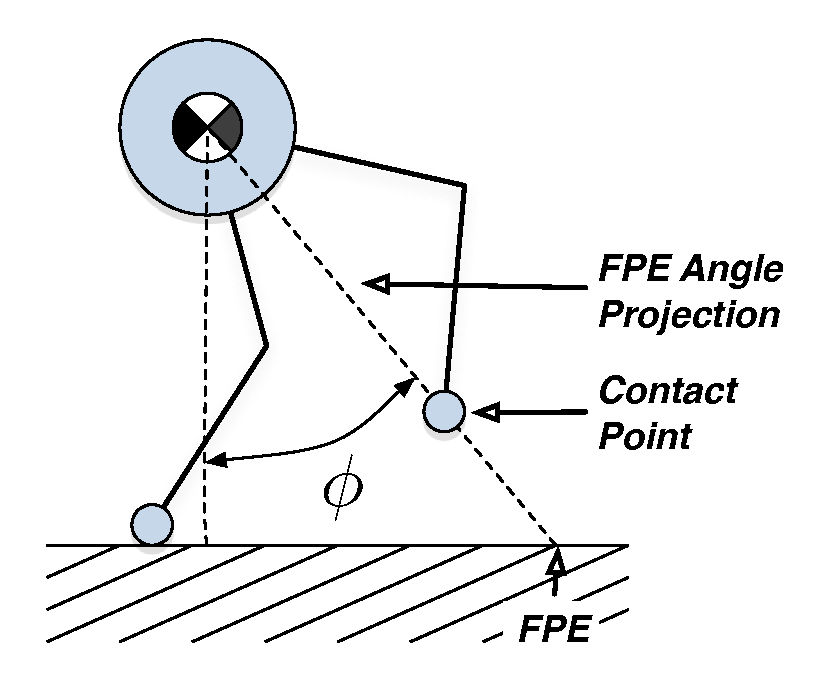
\includegraphics[scale=0.6]{fig/ch4/fpeangle.eps}
  	\caption{Graphical representation of the solution to the FPE equation for arbitrary robot configurations.}
	\label{fig:fpeangle}
\end{figure}

\begin{figure*}[!b]
	\begin{equation} \label{eq:fpe}
	\begin{aligned}
		\frac{{{{\left[ {mh({v_x}\cos \phi  + {v_y}\sin \phi )\cos \phi  + {I_{COM}}{{\dot \theta }_1}{{\cos }^2}\phi } \right]}^2}}}{{m{h^2} + {I_{COM}}{{\cos }^2}\phi }} + 2mgh\cos \phi (\cos \phi  - 1) = 0
	\end{aligned}
	\end{equation}
	\\
	\hrulefill
\end{figure*}

While the stability analysis presented in \cite{Wight:2008ii} considered a simple compass biped, the results of the FPE equation can be extended to any arbitrary planar biped (i.e. with bent knees) by controlling the joint angles of the leg to achieve an equivalent distance $L$ between the COM and the foot contact. If a biped is unstable and begins to pivot forward on a fixed contact point, tracking the angle $\phi$ with the swing foot as the robot falls forward converges to the FPE location when the swing foot hits the ground. Upon impact, the distance between the contact point and the COM would have the the same fixed length $L$ between the contact points and the angle $\phi$ converges to $\beta/2$. The results from the compass biped also extend to the arbitrary biped configuration (i.e. stepping directly on the FPE point results in the kinetic energy being equivalent to the peak potential energy).
% subsection computing_the_fpe_angle (end)

\subsection{Forming Complete Gait Cycles} % (fold)
\label{sub:gait_cycles}
Wight et al. \cite{Wight:2008ii} use the FPE concept to develop full gait cycles using simple linear control techniques and a state machine. Gait is initiated by destabilizing the robot in the desired direction of movement (forward or backward). Once destabilized, the FPE equation is solved numerically to obtain the FPE angle $\phi$, which is used to provide the desired trajectory for the swing foot.  If continued forward progress is desired, the foot is commanded to precede the FPE. If no further forward progress is needed, the foot is commanded to the FPE. The desired trajectory is resolved to joint angles using inverse kinematics and implemented via joint level PD controllers. The complete state machine is shown in Figure~\ref{fig:statemachine}.

\begin{figure}[!h]
	\centering
    \includegraphics[scale=0.22]{fig/ch4/fpestatemachine.png}
  	\caption{A simple state machine used in conjunction with the FPE algorithm to form complete gait cycles}.
	\label{fig:statemachine}
\end{figure}

Due to symmetry, the states in Figure~\ref{fig:statemachine} can be reduced to \textbf{STAND}, \textbf{PUSH}, \textbf{LIFT}, \textbf{SWING} and \textbf{DROP}. For the remainder of this paper, we refer to the sequence of state transitions from \textbf{PUSH} to \textbf{DROP} as a step cycle.
% subsection forming_complete_gait_cycles (end)


% section foot_placement_estimator_in_2d (end)

\section{Extension to 3D} % (fold)
\label{sec:extension_to_3d}

In order to extend the FPE approach to the 3D case, we revisit the concept of generating complete gait cycles described in Section~\ref{sub:gait_cycles}. The primary goal of the first three states in each step cycle (\textbf{PUSH}, \textbf{LIFT} and \textbf{SWING}) is to force the biped into an unstable configuration so that the FPE algorithm can be used to regain stability in the terminal state (\textbf{DROP}).

To extend the 2D algorithm to the general 3D case, we begin by selecting a suitable plane in 3D space as the sagittal plane. The off-sagittal plane is perpendicular to the sagittal plane and the ground.  In the proposed approach, the goal of each step cycle is to control the motion of a 3D bipedal robot to generate a forward moving momentum \emph{along} the selected sagittal plane. Upon entering the terminal state, we solve (\ref{eq:fpe}) on the selected plane to determine the swing foot placement and ultimately regain stability. Unlike the 2D case, we consider a 3D bipedal robot with finite foot length and width rather than a biped with point feet as demonstrated in \cite{Wight:2008ii}. The larger size of the region of support increases robustness to these approximation errors.

The remainder of this thesis assumes a 3D bipedal robot with $n$ actuated degrees of freedom (DOF) and $n+6$ generalized coordinates defined by the following equation of motion:

\begin{eqnarray}
	\label{eq:eom}
	A(\vec{q})\ddot{\vec{q}} + C(\vec{q},\dot{\vec{q}})\dot{\vec{q}} + g(\vec{q}) = \vec{\tau}
\end{eqnarray}

Where $A(\vec{q})$ is the $(n+6) \times (n+6)$ inertia matrix, $C(\vec{q},\dot{\vec{q}})$ are the centripetal/Coriolis terms and $g(\vec{q})$ is the gravity vector. The $(n+6) \times 1$ generalized force vector $\vec{\tau}$ is segmented as follows:

\begin{eqnarray}
	\label{eq:gentau}
	\vec{\tau} = {\begin{bmatrix} \tau_{act} & \tau_{base} \\ \end{bmatrix}}^T
\end{eqnarray}

Where $\tau_{act}$ represents the $n$ actuated DOF and $\tau_{base} = \bf{0}_{6 \times 1} $ are the remaining non-actuated DOF at the floating base.

\subsection{Sagittal Plane} % (fold)
\label{sub:sagittal_plane}
To select an appropriate sagittal plane for a 3D bipedal robot, we choose a vertical plane which lies between the current position of the stance foot and the desired direction of motion. For a 3D biped walking in a forward motion, this plane is chosen as the the vertical plane passing through the midpoint between the hips and parallel to the direction of forward progress. For side-stepping motion, the coronal plane through the stance foot in the direction of the side step is chosen as the sagittal plane.

The motion of the biped is controlled based on the selected plane for the duration of the step cycle. During gait initiation, the lines from the COM to the contact points are of length $L$, and the leg separation angle is $\beta$ (similar to the planar case). If the motion of the biped is constrained along this plane, the FPE angle $\phi$ can be used to determine foot placement to regain stability. The parameters required to compute the 2D FPE along the plane are computed accordingly. That is, the inertia tensor of each link is rotated to obtain the appropriate $I_{COM}$ along the selected sagittal plane.

Upon impact, the angle $\phi$ converges to $\beta/2$ and a new sagittal plane can be selected for the subsequent step cycle prior to the swing leg entering the \textbf{PUSH} state. Once selected, the stance foot is rotated for alignment and swing leg trajectories can be generated along the plane. By selecting a plane between the current and desired directions of motion, our approach can achieve turning with each step.

% subsection sagittal_plane (end)

\subsection{Trajectory Generation} % (fold)
\label{sub:trajectory_generation}
Once the sagittal plane has been identified at the beginning of each step cycle, appropriate task space trajectories must be generated for the COM ($x_{COM}$) and the swing foot ($x_{SWING}$).

% @FIG: diagram of the COM trajectory moving over the stance foot

In the 2D case, the main goal of the initial states \textbf{PUSH}, \textbf{LIFT} and \textbf{SWING} was to achieve enough forward motion to destabilize the biped. In the 3D case, the robot must also remain stable in the off-sagittal plane while achieving the desired sagittal plane motion. If the ZMP leaves the region of support formed by the stance foot as the swing foot is lifted, the biped begins to fall in the off-sagittal plane and the solution to the 2D FPE equation is insufficient to maintain stable gait. To ensure both forward progress and off-sagittal plane stability, the trajectories for the $x_{COM}$ are generated as follows:

\begin{description}
	\item[\textbf{PUSH}] $x_{COM}$ is moved above the leading stance foot to maintain stability in the off-sagittal and sagittal planes.
	\item[\textbf{LIFT}] $x_{COM}$ is held at its current location (above stance foot) while the swing foot is lifted from the ground to achieve sufficient clearance
	\item[\textbf{SWING}] $x_{COM}$ is held in place until the swing foot is aligned with the stance foot in the off-sagittal plane. At this point the $x_{COM}$ is deliberately pushed outside the region of support in the sagittal plane direction.
\end{description}

A similar approach is used to generate trajectories for $x_{SWING}$ to achieve the desired behaviour of generating enough momentum to destabilize the biped in the sagittal plane while maintaining stability in the off-sagittal plane. Trajectories for $x_{SWING}$ are always computed to align with the sagittal plane formed by the stance foot at the start of the step cycle. This ensures that the solution to the 2D FPE equation remains valid as the \textbf{DROP} state is entered.

\begin{description}
	\item[\textbf{PUSH}] $x_{SWING}$ is held in place as the $x_{COM}$ trajectory is tracked.
	\item[\textbf{LIFT}] $x_{SWING}$ follows a ramped trajectory to simultaneously raise the foot off the ground and move it forward in the sagittal plane
	\item[\textbf{SWING}] $x_{SWING}$ follows a straight line trajectory at a specific ground clearance until it reaches the FPE angle $\phi$
\end{description}

The ramp trajectory used to raise the swing foot during \textbf{LIFT} should be parameterized in terms of the velocity of the FPE point so that this state transitions faster in the event of larger disturbances (since the biped would have a shorter amount of time to swing the foot over and catch itself). \\

Depending on the supervisory control mode (i.e. \textbf{WALK} or \textbf{STAND}), the swing leg trajectory can be adjusted to implicitly achieve a desired goal. During \textbf{WALK} mode, the swing foot trajectory tracks a point on the ground slightly behind the FPE point. This under stepping behaviour results in the biped having enough forward moving momentum when the swing foot comes in contact with the ground such that the biped is unstable. As a result, the FPE point is continuously moving forward causing the state machine to transition into the opposing foot's \textbf{LIFT} state upon contact. In the \textbf{STAND} mode, the swing foot trajectory is adjusted to overstep the FPE point so that the biped comes to a stop following this step.

% subsection task_space_trajectory_generation (end)

\subsection{Control Strategy} % (fold)
\label{sub:control_strategy}

A hybrid control strategy is used to simultaneously maintain stability in the off-sagittal plane, achieve sufficient forward momentum along a selected sagittal plane and ultimately track the FPE location to regain stability by taking a step. Similar to the approach presented in \cite{Wight:2008ii}, our approach uses a state machine to transition through the step sequence with each state having a local controller.

During the initial states of the step cycle, whole body motion control is used to track the $x_{COM}$ and $x_{SWING}$ trajectories described in  Section~\ref{sub:trajectory_generation}. To generate the corresponding joint level trajectories, the Jacobian matrix is used to map between the task space and the joint space velocities:

\begin{IEEEeqnarray}{rCl}
	\label{eq:jmap}
	J & = & \begin{bmatrix} \partial q_{act} & \partial x_{base} \\ \end{bmatrix}_{m \times (n+6)}
\end{IEEEeqnarray}

We utilize a prioritized task space control scheme to generate joint level trajectories which simultaneously achieve state goals while satisfying the highest priority constraint (i.e. holding the $x_{COM}$ position). The state-dependent joint level trajectories can be computed by projecting the lower priority task space goals onto the null space of higher priorities:

\begin{eqnarray}
	\label{eq:priori}
	\dot{q}_{ref} = S(J_{H}^{\#} \dot{x}_{H} + N_{H} J_{L}^{\#} \dot{x}_{L})
\end{eqnarray}

Where, $S = \begin{bmatrix} I_{n \times n} & 0_{n \times 6} \\ \end{bmatrix}$ is the actuator selection matrix for (\ref{eq:gentau}), $J^{\#}$ is the psuedoinverse of the Jacobian $J$, $\dot{q}_{ref}$ is the reference joint velocity, and $\dot{x}_H$ and $dot{x}_L$ are the high and low priority task space velocities, respectively. $J_{H}$ are $J_{L}$ are the corresponding high and low priority Jacobians, and $N_{H} = I - J_{H}^{\#} J_{H}$ is the null space projection matrix. The reference joint velocities are integrated to obtain the reference command signal to be tracked by high gain local PD controllers. The specific prioritization of each state is discussed in Section~\ref{sub:joint_level_control}.

When the biped enters the terminal state, our hybrid control strategy switches to directly computing the joint level commands using inverse kinematics. The PD controller gains of the stance foot ankle are set to $K_{P} = K_{D} = 0$ to allow the biped to pivot and fall forward. Simultaneously, the inverse kinematics for the swing leg is solved directly to track the FPE point along the selected sagittal plane.
% subsection control_strategy (end)

\subsection{State Dependent Controllers} % (fold)
\label{sub:joint_level_control}
This section presents the specific controller formulation used during each state of the gait cycle.  \\

\subsubsection{\textbf{STAND}} % (fold)
\label{ssub:stand}
The goal during this state is to maintain the COM position at the geometric centroid of both feet. In order to remain stable under small disturbances, the Jacobian under double support phase is used to compensate for the error $\Delta x_{COM}$ in the X and Y directions.

\begin{IEEEeqnarray}{rClrCl}
	J_{H} & = &
	\begin{bmatrix}
		J_{Stand} \\
		J_{Swing} \\
		J_{COM} \\
	\end{bmatrix}  &
	\dot{x}_{H} & = &
	\begin{bmatrix}
		0 \\
		0 \\
		\dot{x}_{COM} \\
	\end{bmatrix} \nonumber \\
	J_{L} & = &
	\begin{bmatrix}
		0 \\
	\end{bmatrix}  &
	\dot{x}_{L} & = &
	\begin{bmatrix}
		0 \\
	\end{bmatrix} \nonumber \\
\end{IEEEeqnarray}

% subsubsection stand (end)

\subsubsection{\textbf{PUSH}} % (fold)
\label{ssub:push}
The goal during this state is to track the trajectory generated for $x_{COM}$ to move to the stance foot support region while remaining in the double support phase. An augmented Jacobian matrix is used to track the trajectory while simultaneously maintaining the foothold constraints.

\begin{IEEEeqnarray}{rClrCl}
	J_{H} & = &
	\begin{bmatrix}
		J_{Stand} \\
		J_{Swing} \\
		J_{COM} \\
	\end{bmatrix}  &
	\dot{x}_{H} & = &
	\begin{bmatrix}
		0 \\
		0 \\
		\dot{x}_{COM} \\
	\end{bmatrix} \nonumber \\
	J_{L} & = &
	\begin{bmatrix}
		0 \\
	\end{bmatrix}  &
	\dot{x}_{L} & = &
	\begin{bmatrix}
		0 \\
	\end{bmatrix} \nonumber \\
\end{IEEEeqnarray}

The joint level reference velocities are calculated from (\ref{eq:priori}) and integrated to obtain the position command.

% subsubsection push (end)

\subsubsection{\textbf{LIFT}} % (fold)
\label{ssub:lift}
In the lift stage, the highest priority task is maintaining the foothold of the stance foot, holding the $x_{COM}$ directly above it and simultaneously raising the swing foot from the ground. The key challenge in this state is that lifting the swing foot can potentially cause the centre of pressure to leave the support region formed by the contact points of the stance foot. The prioritized task space control scheme is used to generate joint level commands to track the $x_{SWING}$ trajectory while satisfying the higher priority goal of maintaining the foothold and balance.

\begin{IEEEeqnarray}{rClrCl}
	J_{H} & = &
	\begin{bmatrix}
		J_{Stance} \\
		J_{COM} \\
	\end{bmatrix} &
	\dot{x}_{H} & = &
	\begin{bmatrix}
		0 \\
		\dot{x}_{COM} \\
	\end{bmatrix} \nonumber \\
	J_{L} & = &
	\begin{bmatrix}
		J_{Swing} \\
	\end{bmatrix}  &
	\dot{x}_{L} & = &
	\begin{bmatrix}
		\dot{x}_{Swing} \\
	\end{bmatrix} \nonumber \\
\end{IEEEeqnarray}

The joint level reference velocities are calculated from (\ref{eq:priori}) and integrated to obtain the position command. \\

% subsubsection lift (end)

\subsubsection{\textbf{SWING}} % (fold)
\label{ssub:swing}


At this point, the goal of our control approach is to generate a forward moving momentum along the selected sagittal plane. This deliberately destabilizes the biped by pushing $x_{COM}$ outside the region of support in the chosen direction of motion. The task space prioritization in this state remains consistent with the previous state until the biped is unstable, at which point the control strategy enters the terminal \textbf{DROP} state.

\begin{IEEEeqnarray}{rClrCl}
	J_{H} & = &
	\begin{bmatrix}
		J_{Stance} \\
		J_{Swing} \\
	\end{bmatrix} &
	\dot{x}_{H} & = &
	\begin{bmatrix}
		0 \\
		\dot{x}_{Swing} \\
	\end{bmatrix} \nonumber \\
	J_{L} & = &
	\begin{bmatrix}
		J_{COM} \\
	\end{bmatrix}  &
	\dot{x}_{L} & = &
	\begin{bmatrix}
		\dot{x}_{COM} \\
	\end{bmatrix} \nonumber \\
\end{IEEEeqnarray}

The joint level reference velocities are calculated from (\ref{eq:priori}) and integrated to obtain the position command. \\
% subsubsection swing (end)

\subsubsection{\textbf{DROP}} % (fold)
\label{ssub:drop}
In this terminal state, we use the Jacobian to track the fixed stance foot position and the generated swing foot trajectory to track the FPE point on the ground. Since the ZMP is outside of the region of foot support during this state, we treat the torso as a fixed base link and compute the Jacobian matrix of each foot.

\begin{IEEEeqnarray}{rClrCl}
	J_{H} & = &
	\begin{bmatrix}
		J_{Stance} \\
		J_{Swing} \\
	\end{bmatrix} &
	\dot{x}_{H} & = &
	\begin{bmatrix}
		\dot{x}_{Stand} \\
		\dot{x}_{Swing} \\
	\end{bmatrix} \nonumber \\
	J_{L} & = &
	\begin{bmatrix}
		0 \\
	\end{bmatrix}  &
	\dot{x}_{L} & = &
	\begin{bmatrix}
		0 \\
	\end{bmatrix} \nonumber \\
\end{IEEEeqnarray}

By the assumption of an arbitrary 3D biped with finite sized feet, it is possible for the biped to land on the edge of the foot instead of landing perfectly above the FPE point on teh ground. To handle this behaviour, we switch to a stabilization substate where the joint level control is computed directly. At this point, we generate trajectories for the ankles to align the surface of the foot with the ground and switch to high gain PD control for tracking. This ensures that both feet are in full contact with the ground prior to executing the opposite legs gait sequence. \\

% subsubsection drop (end)

% subsection joint_level_control (end)
% section extension_to_3d (end)

\section{Simulations and Results} % (fold)
\label{sec:simulations_and_results}


\subsection{Compass Biped} % (fold)
\label{sub:2d_simulations}

\begin{figure}[!h]
	\begin{center}
	\subfigure{\includegraphics[scale=0.5]{fig/ch4/understeppingtime.eps}}
	\subfigure{\includegraphics[scale=0.5]{fig/ch4/understeppingphase.eps}}
	\end{center}
  	\caption{Time evolution and state trajectories for under stepping (i.e. foot lands behind FPE point)}
	\label{sim:under}
\end{figure}

The compass biped model with the single state variable is simulated to illustrate the effects of overstepping and under stepping. The leg separation angle $\beta$ is held constant and no energy is lost upon impact.

When the biped under steps, the kinetic energy exceeds the potential energy and the biped remains in forward motion (as shown in Figure \ref{sim:under}). Note that a biped using the state machine controller described above would now calculate and track a new FPE angle to restore stability. When the compass biped over steps, the system energy is not high enough to continue forward motion. Instead, the biped rocks back on its hind leg (as shown in Figure \ref{sim:over}).

\begin{figure}[!h]
	\begin{center}
	\subfigure{\includegraphics[scale=0.5]{fig/ch4/oversteppingtime.eps}}
	\subfigure{\includegraphics[scale=0.5]{fig/ch4/oversteppingphase.eps}}
	\end{center}
  	\caption{Time evolution and state trajectories for over stepping (i.e. foot lands in front of FPE point)}
	\label{sim:over}
\end{figure}

% subsection 2d_simulations (end)

\subsection{Side-to-Side Stepping} % (fold)
\label{sub:3d_simulations}

\begin{figure*}[t]
	\centering
    \includegraphics[scale=0.11]{fig/ch4/sequence.png}
  	\caption{Frames from the sequence of motions while side stepping. The gray plane in the frame captures above represents the 2D FPE plane which moves along the Y-direction (biped's frontal plane). The intersection of the gray 2D FPE plane and the ground plane indicate the FPE point tracked during \textbf{DROP}. }
	\label{fig:sequence}
\end{figure*}


The proposed control strategy to extend the FPE theory to 3D was implemented in simulation on a 14 DOF lower body bipedal robot. To demonstrate the dynamic stability of a 3D biped under this approach, the frontal plane was selected as the sagittal plane. Forward motion along this sagittal plane results in a side-to-side stepping sequence for the biped (as shown in Figure \ref{fig:sequence}). Each state of our control strategy was implemented in the Matlab/Simulink environment with the dynamics simulated in SimMechanics. Accurate kinematic and dynamic properties of the physical robot were taken directly from the CAD model \cite{ChoudhuryHumanoids2012}.

\begin{figure}[!h]
	\centering
    \includegraphics[scale=0.5]{fig/ch4/comtraj.eps}
  	\caption{COM trajectory being tracked during the complete gait sequence of side stepping. The colour coded dotted lines indicate the boundaries of each foot on the ground. Note that during the \textbf{SWING} state, the COM is pushed outside the region of support (around 11s). This in turn initiates the \textbf{DROP} state where the FPE point is tracked to regain stability.}
	\label{fig:comtraj}
\end{figure}

The resulting $x_{COM}$ trajectories from simulating the side-to-side stepping motion (shown in Figure \ref{fig:comtraj}) demonstrate the stability of the biped through a complete gait sequence. Our prioritized motion control framework handles the dynamic switching of constraints (from double support to single support) while generating the appropriate joint level commands for swinging the COM over. In the terminal DROP state, the swing foot trajectory tracks the FPE point on the ground (shown in Figure \ref{fig:fpetrack}) with an added offset to ensure that the biped oversteps to guarantee stability (as per the 2D FPE theory). This causes the biped to rock back and forth (similar to the 2D case) until stability is reached.

\begin{figure}[!h]
	\centering
    \includegraphics[scale=0.5]{fig/ch4/fpetrack.eps}
  	\caption{During the \textbf{DROP} state shown here, the swing foot trajectory initially tracks the a point on the ground given by $FPE + FPE_{offset}$ to ensure overstepping. Once ground contact is made (around 11.6s), the stabilization substate is entered and the swing foot trajectory is controlled directly to align the foot with the ground.}
	\label{fig:fpetrack}
\end{figure}

% subsection 3d_simulations (end)

% section simulations_and_results (end)


% chapter simulations (end)